\documentclass[screen, aspectratio=43]{beamer}
\usepackage[T1]{fontenc}
\usepackage[utf8]{inputenc}

% Use the NTNU-temaet for beamer 
% \usetheme[style=ntnu|simple|vertical|horizontal, 
%     language=bm|nn|en, 
%     smalltitle, 
%     city=all|trondheim|alesund|gjovik]{ntnu2017}
\usetheme[style=ntnu,language=en]{ntnu2017}

\usepackage[english]{babel}
\usepackage[style=numeric,backend=biber,natbib=false,sorting=none]{biblatex}
\usepackage{hyperref}

\title[PCW-d1]{Physical Computing Workshop: Day 1}
\subtitle{Intuitive circuits and hacking}
\author[A. Xamb{\'o}]{Anna Xamb{\'o}}
\institute[NTNU]{Department of Music, NTNU}
\date{16 October 2018}
%\date{} % To have an empty date

\addbibresource{../pcw.bib} % Add bibliography database

% Set the reference style to numeric.
% See here: http://tex.stackexchange.com/questions/68080/beamer-bibliography-icon
\setbeamertemplate{bibliography item}[text] 

% Set bibliography fonts to a small size.
\renewcommand*{\bibfont}{\footnotesize}

\begin{document}

\begin{frame}
  \titlepage
\end{frame}
%
\begin{frame}
  \frametitle{Learning Outcomes}
  \begin{itemize}
    \item Identify the fundamental properties of a circuit.
    \item Explore the practice of circuit sniffing using radios, microphones and speakers.
    \item Discover the research and artistic technique of soundwalks.
    \item Discern the fundamental properties of an interactive system.
    \item Get familiar with web technologies (P5.js, javascript).
    \item Be able to adapt javascript code of a sampler with custom recordings. 
    \item Demonstrate a custom-made sampler instrument in a performance setting.
    \item Reflect on the custom-made sampler instrument and performance using a blogging style.
    \end{itemize}
\end{frame}
%
\begin{frame}
  \frametitle{Preparation: Reading + Questionnaire}
        \begin{itemize}
        \item Read / skim through the following article and be ready to discuss it in class:
         \begin{itemize}
         \item Collins, N. (2004) The Seven Rules of Hacking (chapter 2):\\
         \url{http://www.nicolascollins.com/texts/originalhackingmanual.pdf}
         \item  Adams, M.D. et al. (2008) ``Soundwalking as a methodology for understanding soundscapes'':\\
         \url{http://usir.salford.ac.uk/2461/1/Adams_etal_2008_Soundwalking_as_Methodology.pdf}
         \end{itemize}
        \item Fill in the following questionnaire before coming to class: \\
 	\url{https://goo.gl/gW6XEm}       
         \end{itemize}
\end{frame}
%
\begin{frame}
  \frametitle{Preparation: What to Bring to Class?}
        \begin{itemize}
        \item Cheap headphones / earplugs.
        \item A mobile phone with a radio program or a battery-powered AM radio.
        \item A minijack to jack adapter.
        \item Extra 9V batteries.
        \item A battery-powered amplifier (optional, you will have 1 per group).
        \item Any type of contact mic, pickup or piezo (optional, you will have 1 per group).
         \end{itemize}
\end{frame}
%
\begin{frame}
  \frametitle{Preparation: What We Do Provide?}
        \begin{itemize}
        \item A handout: \url{XXX}..
        \item A spreadsheet for block I: circuit sniffing and soundwalking activities: \url{XXX}..
        \item 3 mini amps.
        \item 3 piezo transducer pickups.
        \item 7 Music Angel speakers for the performance.
        \item Slides: \url{XXX}.
        \item Code: \url{XXX}..
         \end{itemize}
\end{frame}
%
\begin{frame}
  \frametitle{Outline}
      \begin{itemize}
	\item Block I: Circuit sniffing + soundwalking activities
	\item Block II: Basic interactive behavior activities: building a sampler around the morning's audio recordings
	\item Block III: Rehearsal and performance
    \end{itemize}  
\end{frame}
%
\begin{frame}
  \frametitle{Pre-knowledge Activity: Soundwalks}
  Be ready to discuss about soundwalking from the suggested reading.
\end{frame}
%
\begin{frame}
  \frametitle{Block I: Circuit sniffing + soundwalking activities}
        \begin{itemize}
	\item Combination of soundwalks and circuit sniffing.
	\item Mapping of materials / situations that work for different conditions (filling in the provided spreadsheet).
	\item Generation of audio recordings for later use.
	\item Distribution of work between group members in the wild and group members in the ``station''. 
	\item Each group will present their results for one of the soundwalk activities.
	\item This material will be used for the daily blog.
    \end{itemize} 
\end{frame}
%
\begin{frame}
  \frametitle{The seven basic rules of hacking (Collins 2006)}
        \begin{itemize}
	\item Rule \#1: Fear not!
	\item Rule \#2: Don't take apart anything that plugs directly into the wall.
	\item Rule \#3: It is easier to take something apart than put it back together.
	\item Rule \#4: Make notes of what you are doing as you go along, not after.
	\item Rule \#5: Avoid connecting the battery backwards.
	\item Rule \#6: Many hacks are like butterfies: beautiful but short-lived.
	\item Rule \#7: In general, try to avoid short circuits.
    \end{itemize} 
\end{frame}
%
\begin{frame}
  \frametitle{Exercise 1: Radios and interferences}
   \begin{figure}
	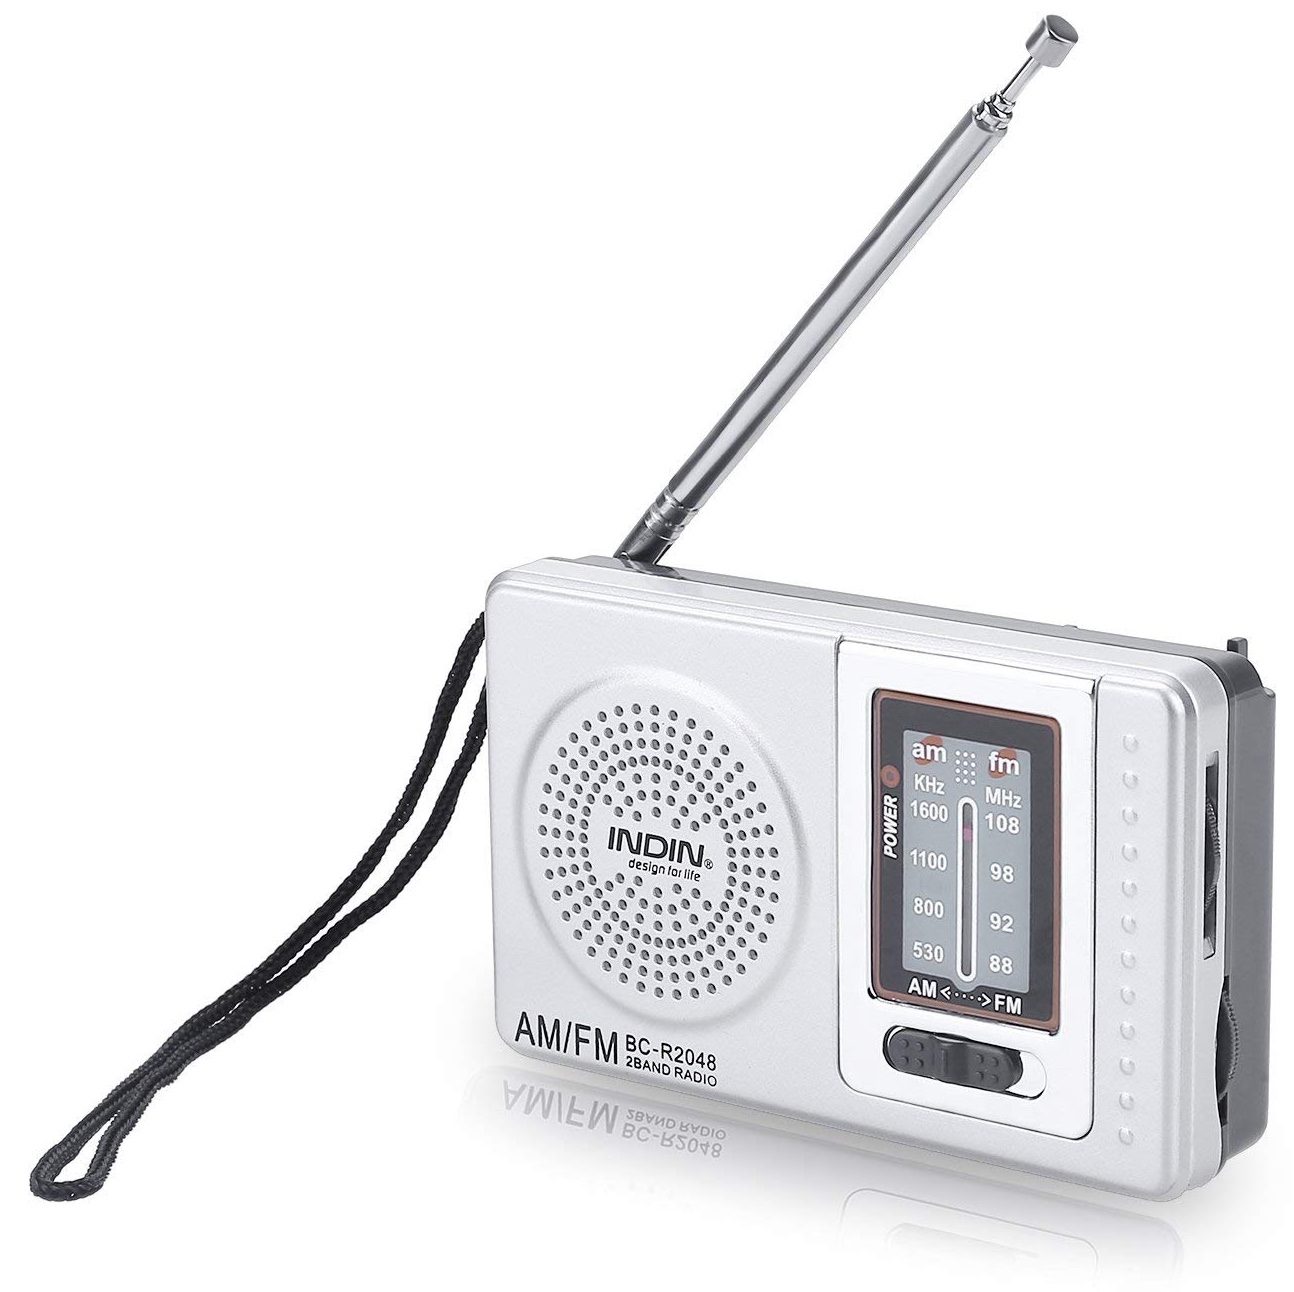
\includegraphics[scale=0.09]{img/battery-powered-radio.jpg}
\end{figure}
{\scriptsize 
Radios pick up electromagnetic waves and translate them into signals that can be heard through the loudspeaker.
    \begin{itemize}
	\item Go for a soundwalk with a radio using the circuit sniffing technique and try moving it around various electrical appliances (e.g. fluorescent lights, infrared remote controls, computers...).
	\item Annotate on the spreadsheet and record what is interesting.
    \end{itemize}   
}    
{\tiny
Exercise based on ``Chapter 3. Circuit sniffing: using radios and coils to eavesdrop on hidden electromagnetic music'' (Collins 2006).
}
\end{frame}
%
\begin{frame}
  \frametitle{Exercise 2: Speaker as a microphone}
 \begin{figure}
	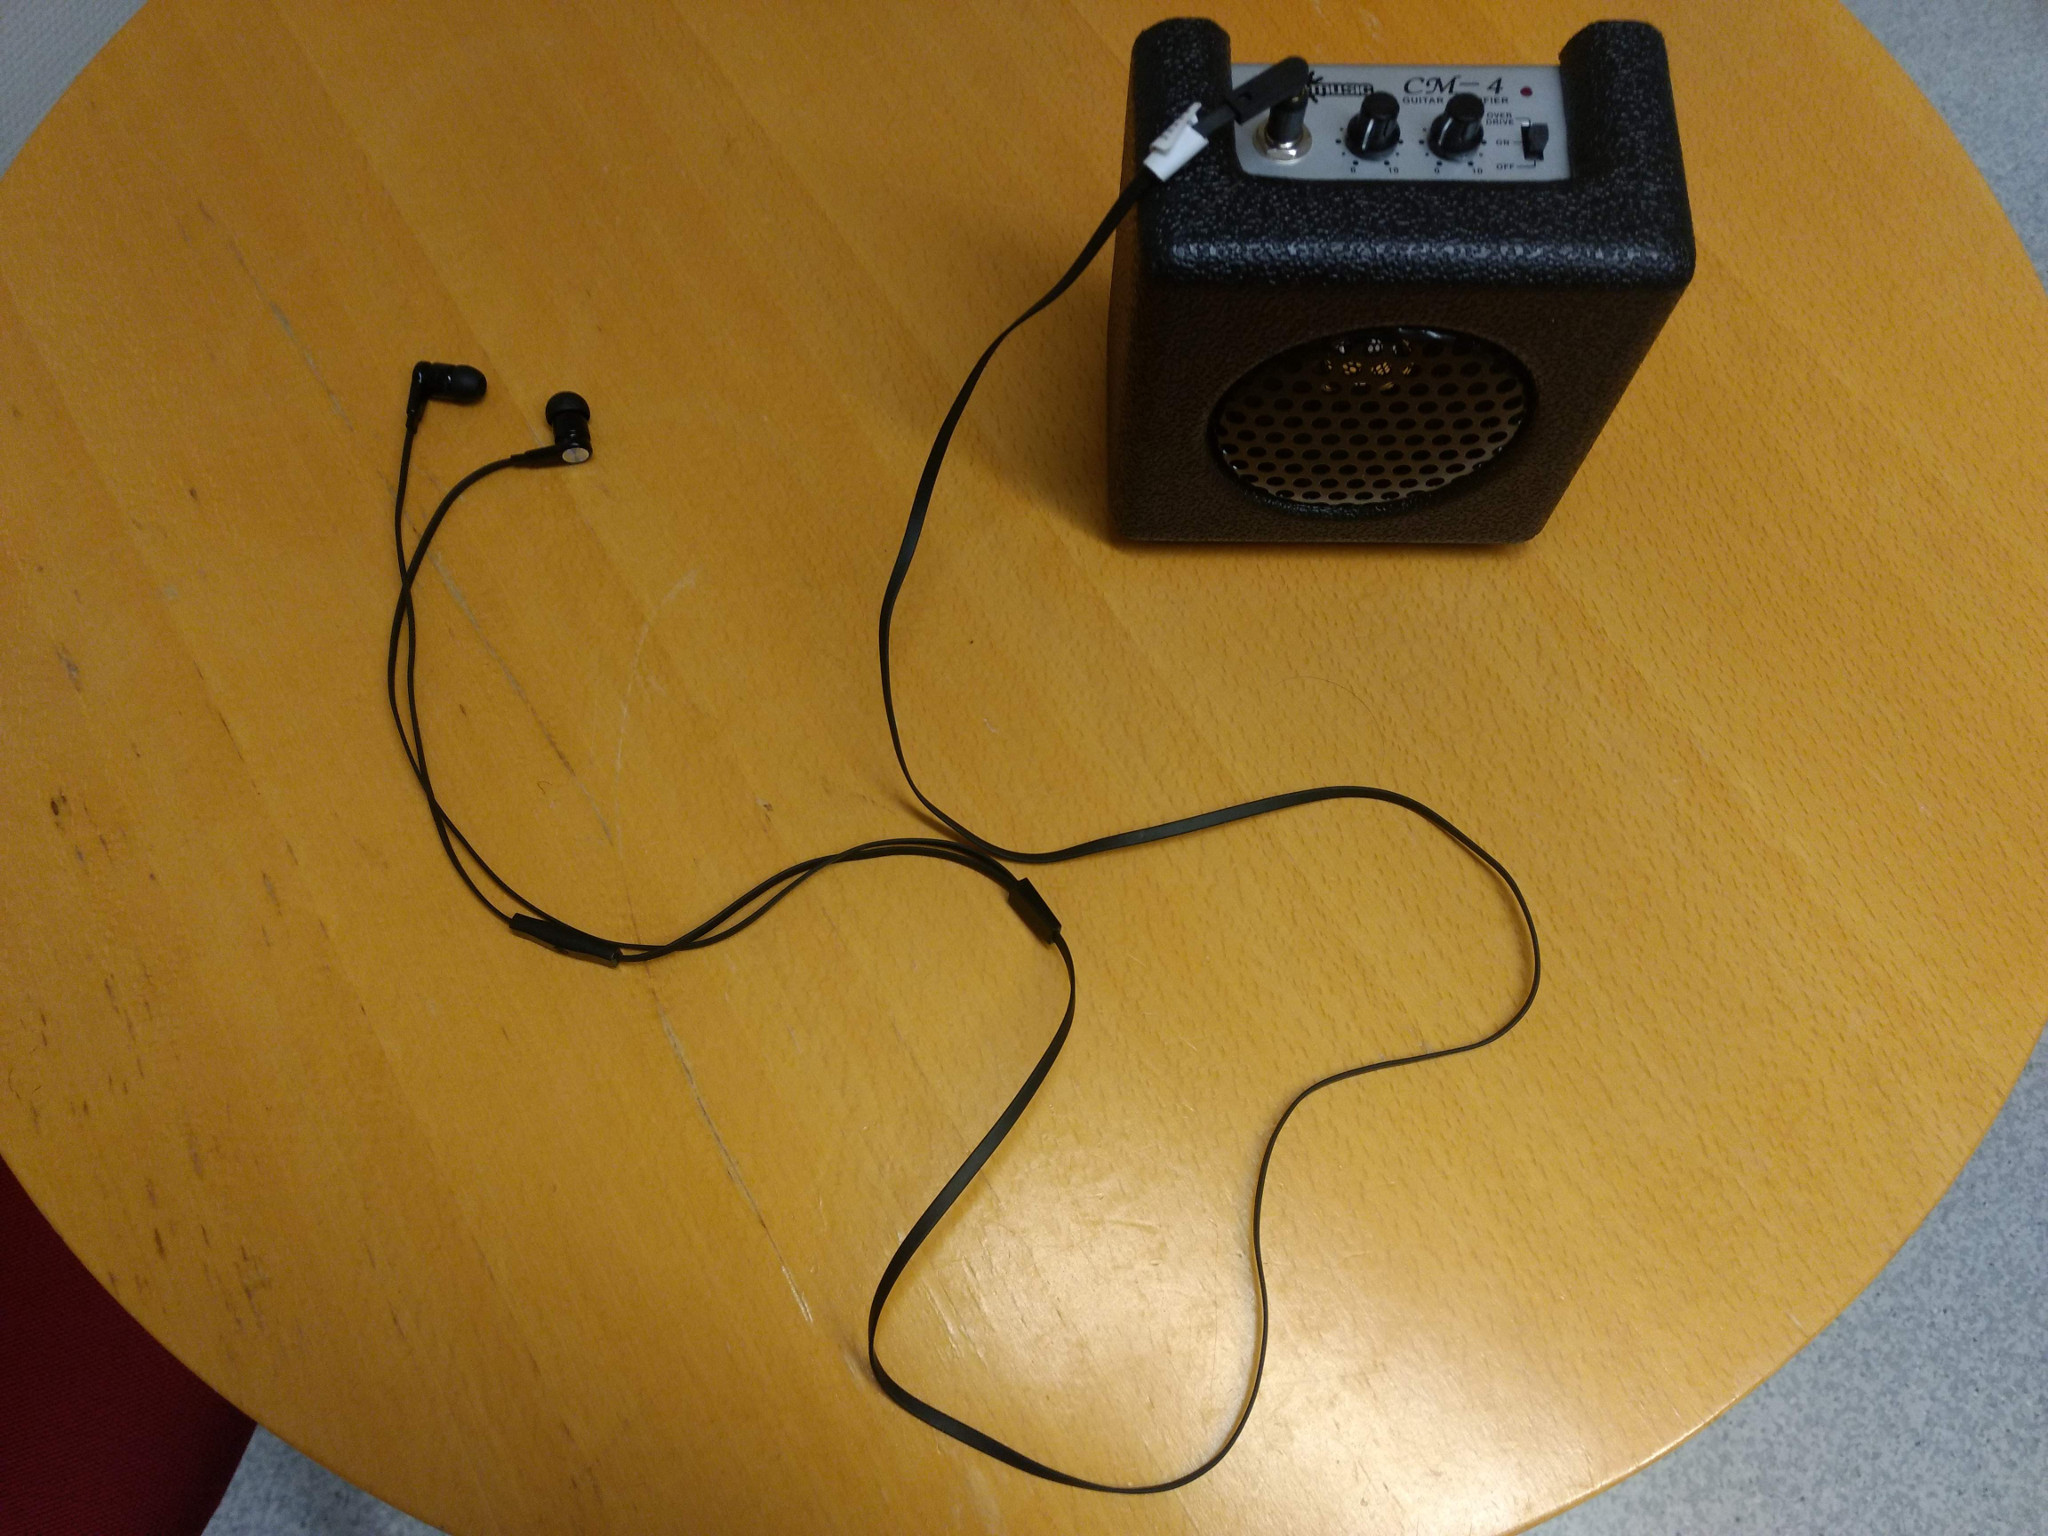
\includegraphics[scale=0.05]{img/coilsamps.jpg}
\end{figure}
{\scriptsize 
Headphones are tiny speakers (both have coils and magnets to transform acoustic sound into an electrical signal or the other way around). The same electromagnetic force is used for both microphones and speakers.
    \begin{itemize}
	\item Go for a soundwalk with headphones as speakers using the circuit sniffing technique.    
	\item Annotate on the spreadsheet and record what is interesting.
    \end{itemize}
 }   
    {\tiny Exercise based on:
     \begin{itemize}
    	\item ``Chapter 4. In/out (the eight rule of hacking): speaker as microphone, microphone as speaker -- the symmetry of it all'' (Collins 2006)
	\item Video ``Tutorial 2: In/Out - Electromagnetism Explained (Chapter 4)'' (source: www.nicolascollins.com)\\ 
	\url{https://www.nicolascollins.com/video/tutorial02/tutorial02-desktop.m4v} 
      \end{itemize}	
    }
       
\end{frame}
%
\begin{frame}
  \frametitle{Exercise 3: Contact mics and amps}
 \begin{figure}
	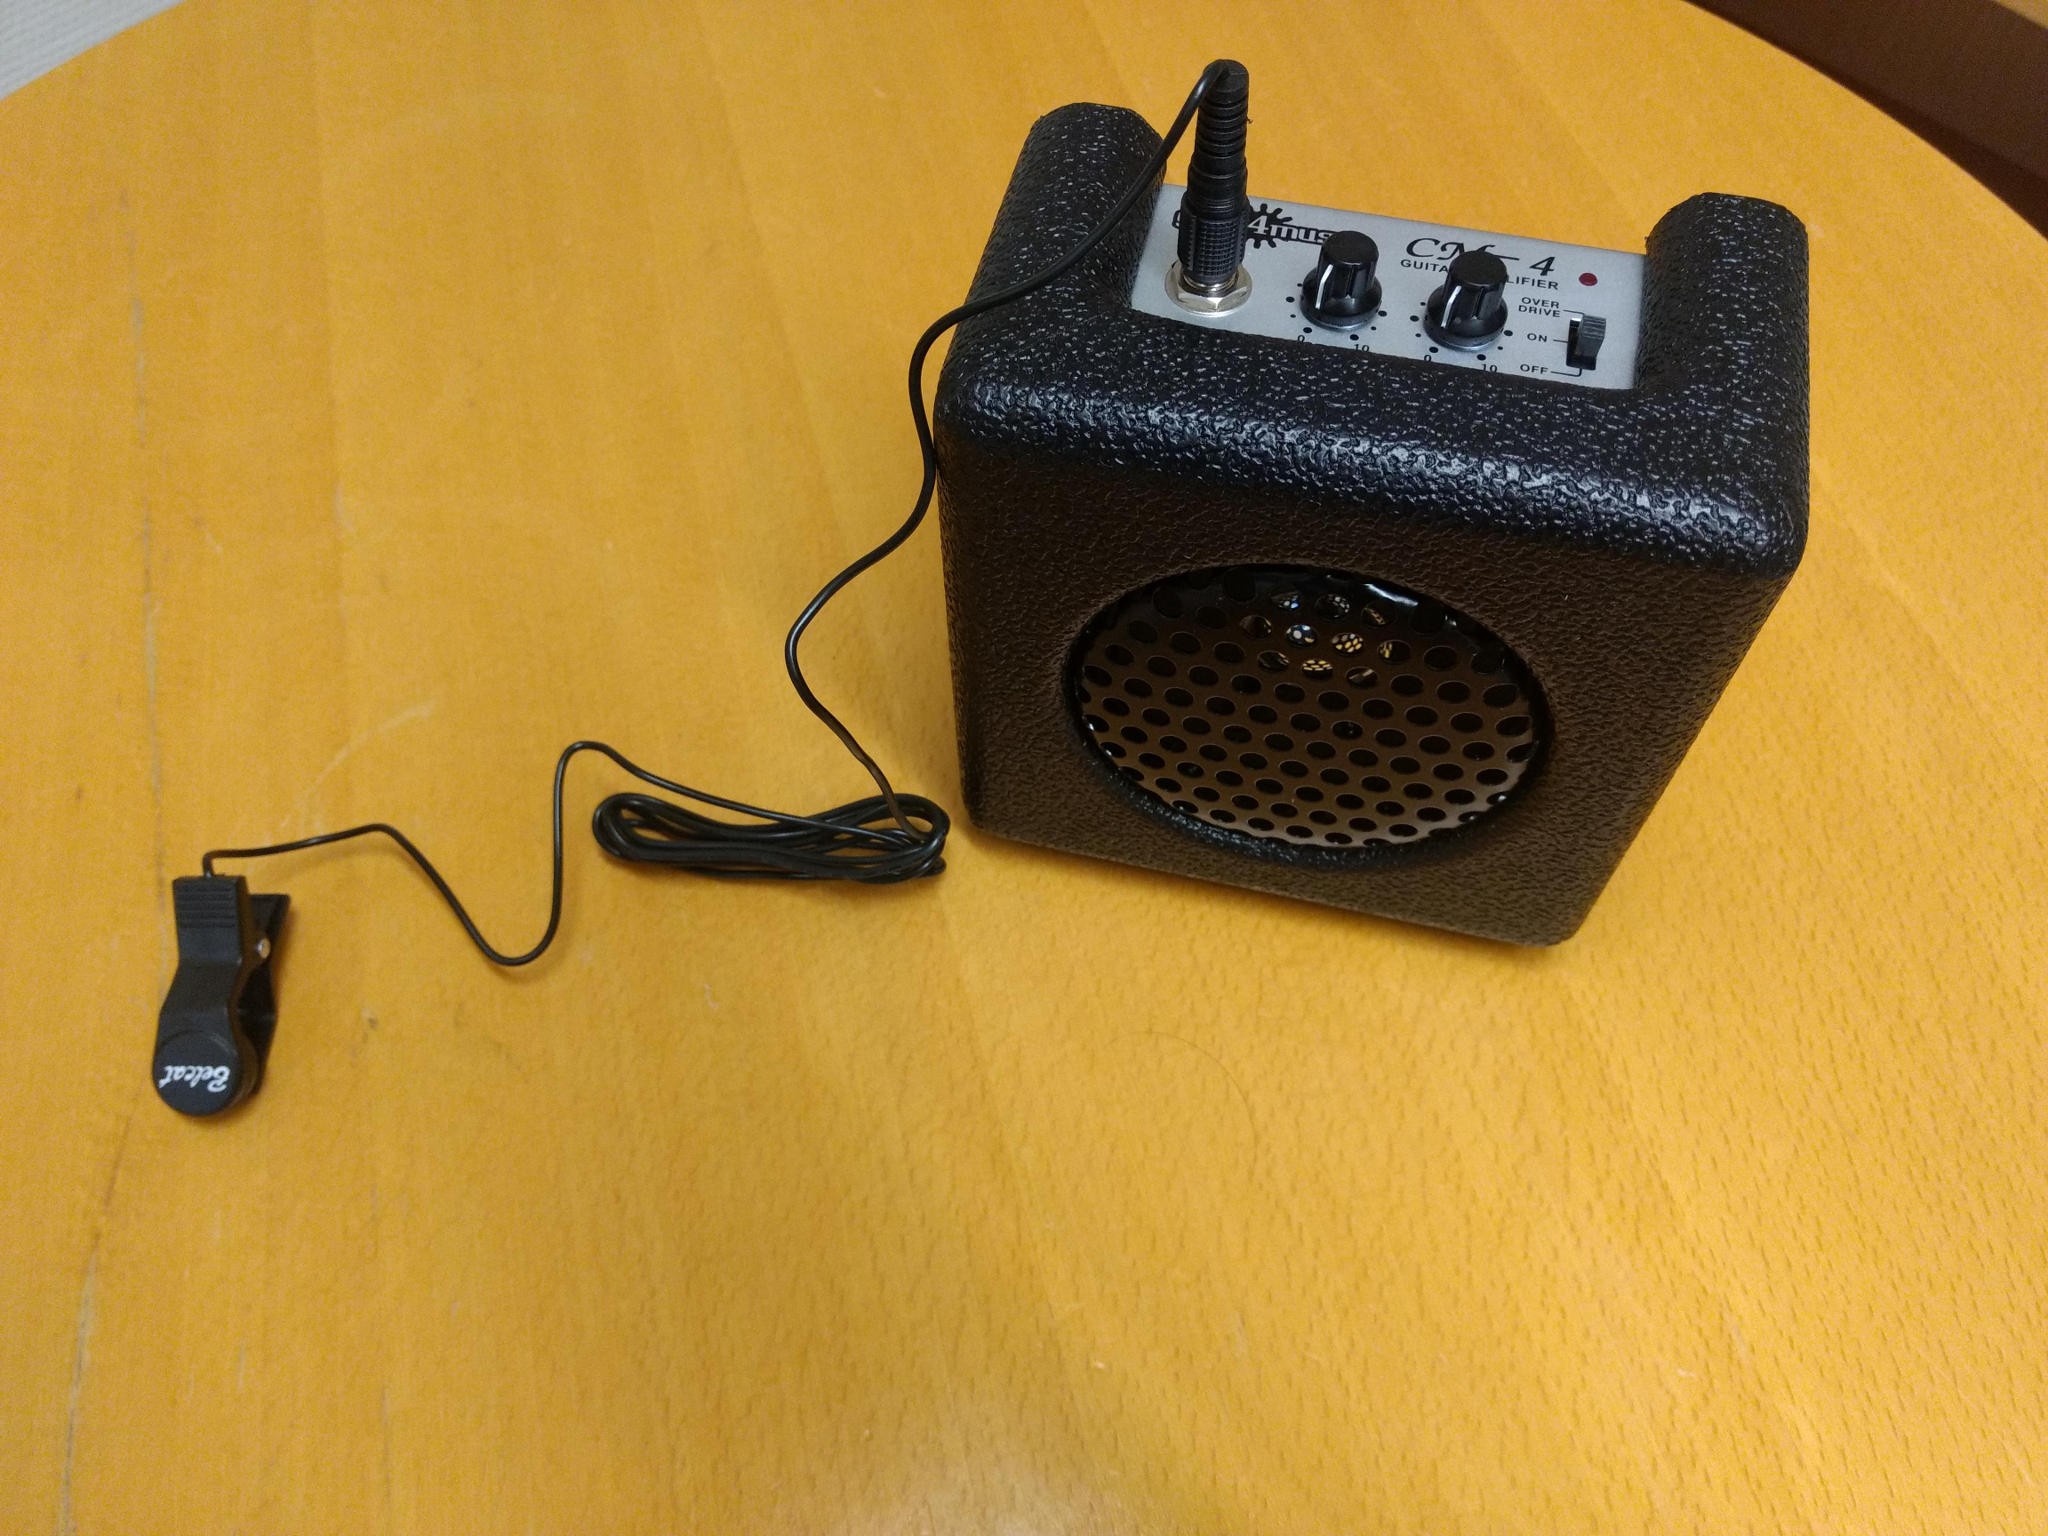
\includegraphics[scale=0.05]{img/contactmics.jpg}
\end{figure}  

  {\scriptsize 
  A contact mic, also known as a pickup or piezo, is a form of microphone that senses audio vibrations through contact with solid objects.
  \begin{itemize}
    \item Go for a soundwalk with contact mics and amps using the circuit sniffing technique.    
    \item Annotate on the spreadsheet and record what is interesting.
  \end{itemize}
  }
  {\tiny Exercise based on:	  
    \begin{itemize}
	\item ``Chapter 3. Circuit sniffing: using radios and coils to eavesdrop on hidden electromagnetic music'' (Collins 2006)
	\item Video ``Tutorial 1: Circuit Sniffing (Chapter 3)'' (source: www.nicolascollins.com)\\ 
	\url{https://www.nicolascollins.com/video/tutorial01/tutorial01-desktop.m4v}
	\item Video ``Tutorial 5: How to Make a Contact Mike (Chapter 7)'' (source: www.nicolascollins.com)\\
	\url{https://www.nicolascollins.com/video/tutorial05/tutorial05-desktop.m4v}
    \end{itemize}
   } 
\end{frame}
%
\begin{frame}
  \frametitle{Exercise 4: Install P5.js and ``Hello, World''}
 Exercise: Download and familiarize with the code from ``P5\_01\_hello\_world'' project. Print ``Hello, World'' to the javascript console.
 Each student should have a laptop/terminal. In each terminal there should be installed:
    \begin{itemize}
	\item A code editor (e.g. Atom, Sublime...).
	\item A browser.
	\item Python to run a simple local server (as explained here: \url{https://github.com/processing/p5.js/wiki/Local-server}).
	\item Internet.
	\item Optionally: Headphones (if we want to avoid disturbing the other students).
	\item For each project it will be included P5.js library including p5.sound.js.
    \end{itemize}
\end{frame}
%
\begin{frame}
  \frametitle{Exercise 5: A simple sampler in P5.js}
  Go through the code and exercises from: 
   \begin{itemize}
  	\item ``P5\_02\_loadSound''
	\item ``P5\_03\_loadSound\_playstop\_keyboard'' 
	\item ``P5\_04\_loadSound\_play\_four\_sounds''
   \end{itemize}
  
  
\end{frame}
%
\begin{frame}
  \frametitle{Exercise 6: A customized sampler in P5.js}
  Create your own sampler with today's recordings. Be ready to perform with it!
\end{frame}
%
\begin{frame}
  \frametitle{Resources: Soundwalks}
    \begin{itemize}
	\item Soundwalking as a methodology for understanding soundscapes (paper)\\ 
	\url{http://usir.salford.ac.uk/2461/1/Adams_etal_2008_Soundwalking_as_Methodology.pdf}
    \end{itemize}    
\end{frame}
%
\begin{frame}
  \frametitle{Resources: Circuits}
    \begin{itemize}
    \item Basic electricity - What is an ampere / amp? (video): \url{https://www.youtube.com/watch?v=8gvJzrjwjds}
    \item Circuit fundamentals (video): \url{https://www.youtube.com/watch?v=MusUypbX73Y}
    %\item How to measure and debug a circuit?
    %\item Conductive vs non-conductive materials, effects current flow
    %\item How to draw a circuit? (symbols)
    %\item Ohm's Law Calculator
    \end{itemize}    
\end{frame}
%
\begin{frame}
  \frametitle{Resources: Contact mics}
    \begin{itemize}
    	\item Different Types of Transducers in Practical Applications: \url{https://www.efxkits.com/blog/different-types-of-transducers-in-practical-applications/}
	\item The first rule of CONTACT MIC club: \url{http://www.musicofsound.co.nz/blog/the-first-rule-of-contact-mic-club}
	\item 9 ways to use piezo mics in your music making: \url{https://www.musicradar.com/tuition/tech/9-ways-to-use-piezo-mics-in-your-music-making-627533}
	\item Building contact mics: \url{http://maaheli.ee/main/building-contact-microphones/}
	\item How to use a contact mic for sound design: \url{http://www.synthtopia.com/content/2016/08/15/how-to-use-a-contact-mic-for-sound-design/}
    \end{itemize}    
\end{frame}
%
\begin{frame}
  \frametitle{Other Resources: Engineering}
    \begin{itemize}
    \item What is Electrical Engineering? \url{https://www.youtube.com/watch?v=QQewdCJTcIU}
    \item Inspiring the next generation of female engineers \url{https://www.youtube.com/watch?v=FEeTLopLkEo}
    \end{itemize}
\end{frame}
%
\begin{frame}
  \frametitle{Other Resources: How to Solder}
    \begin{itemize}
    \item ``Chapter 6. How to solder? An essential skill'' (Collins 2006)\\
    \url{https://www.nicolascollins.com/video/tutorial04/tutorial04-desktop.m4v}     
    \item How to solder? (video) (source: www.nicolascollins.com)\\
    \url{https://www.nicolascollins.com/video/tutorial04/tutorial04-desktop.m4v} 
    \end{itemize}
\end{frame}
%
\begin{frame}
  \frametitle{Other Resources: Listening}
    \begin{itemize}
    \item ``Tutorial 3: Jumping Speakers (Chapter 5)'' (source: www.nicolascollins.com)\\
    \url{https://www.nicolascollins.com/video/tutorial03/tutorial03-desktop.m4v}
    \item Alvin Lucier's (USA) ``Sferics'' (1980)\\
    Audio: \url{https://www.youtube.com/watch?v=rxUvMl_IxoQ}\\
    About: \url{http://www.alvin-lucier-film.com/sferics.html}
    \item Karlheinz Stockhausen (Germany), ``Kurzwellen'' (1968) used four receivers in live performance\\
    Audio: \url{https://www.youtube.com/watch?v=uQ_vGr9U3QY}
    \item ``Pack: contact microphone recordings'' by klankbeeld\\
    \url{https://freesound.org/people/klankbeeld/packs/11282/}
    \end{itemize}
\end{frame}
%
\begin{frame}
  \frametitle{Other Resources: Listening II}
    \begin{itemize}
    \item ``Storytable'' by composer Gyrid Nordal Kaldestad, performed by Architek Percussion (Ben Duinker, Mark Morton, Ben Reimer, Alessandro Valiante):\\
    \url{https://vimeo.com/184034352}
    \item Owen Green and his work on cardboard boxes. \\
    ``Neither the Time Nor the Energy'' (Electric Spring 2018): \url{https://www.youtube.com/watch?v=VExDlHD7o80}
    \end{itemize}
\end{frame}
%
%\begin{frame}
%  \frametitle{References}
%  \printbibliography
%\end{frame}
%
\end{document}
